
\documentclass[conference]{IEEEtran}
% *** MISC UTILITY PACKAGES ***
%
%\usepackage{ifpdf}
\usepackage{float}  % For handling float environments like [H]
\usepackage{url}    % For handling URLs
\usepackage{multirow}
\usepackage[caption=false]{subfig}
%\usepackage{subcaption} % Required for subfigures
% Heiko Oberdiek's ifpdf.sty is very useful if you need conditional
% compilation based on whether the output is pdf or dvi.
% usage:
% \ifpdf
%   % pdf code
% \else
%   % dvi code
% \fi
% The latest version of ifpdf.sty can be obtained from:
% http://www.ctan.org/pkg/ifpdf
% Also, note that IEEEtran.cls V1.7 and later provides a builtin
% \ifCLASSINFOpdf conditional that works the same way.
% When switching from latex to pdflatex and vice-versa, the compiler may
% have to be run twice to clear warning/error messages.


\usepackage{cite}
\pagestyle{plain}

% *** GRAPHICS RELATED PACKAGES ***
%
\ifCLASSINFOpdf
  \usepackage[pdftex]{graphicx}
  % declare the path(s) where your graphic files are
  % \graphicspath{{../pdf/}{../jpeg/}}
  % and their extensions so you won't have to specify these with
  % every instance of \includegraphics
  % \DeclareGraphicsExtensions{.pdf,.jpeg,.png}
\else
  % or other class option (dvipsone, dvipdf, if not using dvips). graphicx
  % will default to the driver specified in the system graphics.cfg if no
  % driver is specified.
  % \usepackage[dvips]{graphicx}
  % declare the path(s) where your graphic files are
  % \graphicspath{{../eps/}}
  % and their extensions so you won't have to specify these with
  % every instance of \includegraphics
  % \DeclareGraphicsExtensions{.eps}
\fi
% graphicx was written by David Carlisle and Sebastian Rahtz. It is
% required if you want graphics, photos, etc. graphicx.sty is already
% installed on most LaTeX systems. The latest version and documentation
% can be obtained at: 
% http://www.ctan.org/pkg/graphicx
% Another good source of documentation is "Using Imported Graphics in
% LaTeX2e" by Keith Reckdahl which can be found at:
% http://www.ctan.org/pkg/epslatex
%
% latex, and pdflatex in dvi mode, support graphics in encapsulated
% postscript (.eps) format. pdflatex in pdf mode supports graphics
% in .pdf, .jpeg, .png and .mps (metapost) formats. Users should ensure
% that all non-photo figures use a vector format (.eps, .pdf, .mps) and
% not a bitmapped formats (.jpeg, .png). The IEEE frowns on bitmapped formats
% which can result in "jaggedy"/blurry rendering of lines and letters as
% well as large increases in file sizes.
%
% You can find documentation about the pdfTeX application at:
% http://www.tug.org/applications/pdftex





% *** MATH PACKAGES ***
%
\usepackage{amsmath}
% A popular package from the American Mathematical Society that provides
% many useful and powerful commands for dealing with mathematics.
%
% Note that the amsmath package sets \interdisplaylinepenalty to 10000
% thus preventing page breaks from occurring within multiline equations. Use:
%\interdisplaylinepenalty=2500
% after loading amsmath to restore such page breaks as IEEEtran.cls normally
% does. amsmath.sty is already installed on most LaTeX systems. The latest
% version and documentation can be obtained at:
% http://www.ctan.org/pkg/amsmath





% *** SPECIALIZED LIST PACKAGES ***
%
%\usepackage{algorithmic}
% algorithmic.sty was written by Peter Williams and Rogerio Brito.
% This package provides an algorithmic environment fo describing algorithms.
% You can use the algorithmic environment in-text or within a figure
% environment to provide for a floating algorithm. Do NOT use the algorithm
% floating environment provided by algorithm.sty (by the same authors) or
% algorithm2e.sty (by Christophe Fiorio) as the IEEE does not use dedicated
% algorithm float types and packages that provide these will not provide
% correct IEEE style captions. The latest version and documentation of
% algorithmic.sty can be obtained at:
% http://www.ctan.org/pkg/algorithms
% Also of interest may be the (relatively newer and more customizable)
% algorithmicx.sty package by Szasz Janos:
% http://www.ctan.org/pkg/algorithmicx




% *** ALIGNMENT PACKAGES ***
%
%\usepackage{array}
% Frank Mittelbach's and David Carlisle's array.sty patches and improves
% the standard LaTeX2e array and tabular environments to provide better
% appearance and additional user controls. As the default LaTeX2e table
% generation code is lacking to the point of almost being broken with
% respect to the quality of the end results, all users are strongly
% advised to use an enhanced (at the very least that provided by array.sty)
% set of table tools. array.sty is already installed on most systems. The
% latest version and documentation can be obtained at:
% http://www.ctan.org/pkg/array


% IEEEtran contains the IEEEeqnarray family of commands that can be used to
% generate multiline equations as well as matrices, tables, etc., of high
% quality.




% *** SUBFIGURE PACKAGES ***
%\ifCLASSOPTIONcompsoc
%  \usepackage[caption=false,font=normalsize,labelfont=sf,textfont=sf]{subfig}
%\else
%  \usepackage[caption=false,font=footnotesize]{subfig}
%\fi
% subfig.sty, written by Steven Douglas Cochran, is the modern replacement
% for subfigure.sty, the latter of which is no longer maintained and is
% incompatible with some LaTeX packages including fixltx2e. However,
% subfig.sty requires and automatically loads Axel Sommerfeldt's caption.sty
% which will override IEEEtran.cls' handling of captions and this will result
% in non-IEEE style figure/table captions. To prevent this problem, be sure
% and invoke subfig.sty's "caption=false" package option (available since
% subfig.sty version 1.3, 2005/06/28) as this is will preserve IEEEtran.cls
% handling of captions.
% Note that the Computer Society format requires a larger sans serif font
% than the serif footnote size font used in traditional IEEE formatting
% and thus the need to invoke different subfig.sty package options depending
% on whether compsoc mode has been enabled.
%
% The latest version and documentation of subfig.sty can be obtained at:
% http://www.ctan.org/pkg/subfig




% *** FLOAT PACKAGES ***
%
%\usepackage{fixltx2e}
\usepackage{float}
% fixltx2e, the successor to the earlier fix2col.sty, was written by
% Frank Mittelbach and David Carlisle. This package corrects a few problems
% in the LaTeX2e kernel, the most notable of which is that in current
% LaTeX2e releases, the ordering of single and double column floats is not
% guaranteed to be preserved. Thus, an unpatched LaTeX2e can allow a
% single column figure to be placed prior to an earlier double column
% figure.
% Be aware that LaTeX2e kernels dated 2015 and later have fixltx2e.sty's
% corrections already built into the system in which case a warning will
% be issued if an attempt is made to load fixltx2e.sty as it is no longer
% needed.
% The latest version and documentation can be found at:
% http://www.ctan.org/pkg/fixltx2e


%\usepackage{stfloats}
% stfloats.sty was written by Sigitas Tolusis. This package gives LaTeX2e
% the ability to do double column floats at the bottom of the page as well
% as the top. (e.g., "\begin{figure*}[!b]" is not normally possible in
% LaTeX2e). It also provides a command:
%\fnbelowfloat
% to enable the placement of footnotes below bottom floats (the standard
% LaTeX2e kernel puts them above bottom floats). This is an invasive package
% which rewrites many portions of the LaTeX2e float routines. It may not work
% with other packages that modify the LaTeX2e float routines. The latest
% version and documentation can be obtained at:
% http://www.ctan.org/pkg/stfloats
% Do not use the stfloats baselinefloat ability as the IEEE does not allow
% \baselineskip to stretch. Authors submitting work to the IEEE should note
% that the IEEE rarely uses double column equations and that authors should try
% to avoid such use. Do not be tempted to use the cuted.sty or midfloat.sty
% packages (also by Sigitas Tolusis) as the IEEE does not format its papers in
% such ways.
% Do not attempt to use stfloats with fixltx2e as they are incompatible.
% Instead, use Morten Hogholm'a dblfloatfix which combines the features
% of both fixltx2e and stfloats:
%
% \usepackage{dblfloatfix}
% The latest version can be found at:
% http://www.ctan.org/pkg/dblfloatfix




% *** PDF, URL AND HYPERLINK PACKAGES ***
%
%\usepackage{url}
% url.sty was written by Donald Arseneau. It provides better support for
% handling and breaking URLs. url.sty is already installed on most LaTeX
% systems. The latest version and documentation can be obtained at:
% http://www.ctan.org/pkg/url
% Basically, \url{my_url_here}.



% correct bad hyphenation here
\hyphenation{op-tical net-works semi-conduc-tor}


\begin{document}


\title{Applying ML to assess fatigue and prevent injury\\in high performance swimming athletes}


% author names and affiliations
% use a multiple column layout for up to three different
% affiliations
\author{\IEEEauthorblockN{Hugo Veríssimo}
\IEEEauthorblockA{Foundations of Machine Learning 24/25\\
University of Aveiro\\
Aveiro, Portugal\\
hugoverissimo@ua.pt}
\and
\IEEEauthorblockN{João Cardoso}
\IEEEauthorblockA{Foundations of Machine Learning 24/25\\
University of Aveiro\\
Aveiro, Portugal\\
joaopcardoso@ua.pt}}
% use for special paper notices
%\IEEEspecialpapernotice{(Invited Paper)}




% make the title area
\maketitle
\thispagestyle{plain}

% As a general rule, do not put math, special symbols or citations
% in the abstract
\begin{abstract}
temos que arranjar refs para ir metendo por ai
\end{abstract}


\IEEEpeerreviewmaketitle


\section{Introduction}
The evolution in performance of high level athletes is highly dependent on their skill, motivation, and discipline. With the support of a knowledgeable coach, the evolution can be substantially improved, through careful tailoring of the training regimen. One of the most relevant metrics since the dawn of structure training in sports is the feedback from the athlete, commonly described as the rate of perceived exertion (RPE). This single metric comprises the athletes analysis and intuition of the effort that was carried and how ready they feel for another bout of training. In recent years, more and more sports coaches have relied heavily on collected data to better assess, plan and adjust the training plans of their athletes in a systematic way. This allows for a fine balance between intense workouts, that generate stronger stimuli for muscle development and sport specific skills, taking the balance between effort and fatigue as the crucial ratio to respect. Too high effort, may lead to injury, too low and some gains may be left on the table. 

In the scope of the first project for Foundations of Machine Learning, we decided to partner with the local sports club CAPGE (Clube Associação de Pais da Gafanha da Encarnação) to treat the data (kindly shared by Sr Coach Daniel Tavares) for estimating the fatigue of several athletes. The data was curated and prepared to implement and fit several machine learning algorithms to estimate fatigue after workout.

With this approach, we aim to generalize the models for different athletes/sports, and make it available to the local club for implementation and further testing. 



\section{State of the Art}

Over the past decade there have been significant improvements in the field of ML applied algorithms for sports' related applications. Here we present the most relevant work in fatigue and injury prediction, which is not specifically on the sport we're assessing in our dataset, which lead to additional interpretations from the works analyzed to our own case of study. In general, the problem of class imbalance is seen throughout the literature, and different solutions are proposed, such as data gathering and preprocessing, over sampling and under sampling, with SMOTE (synthetic minority over-sampling technique) being the most commonly used approach for over sampling. As early as 2010, Gabbet and colleagues modeled the risk of injury with a monodimensional approach using logistic regression, based on athletes rate of perceived exertion, showing that even with a monovariate approach to injury prediction useful results could be attained. In recent years, several authors have focused in alternative techniques such as Logistic Regression, Random Forest, Support Vector Machine, or Convolutional Neural Network on Multivariate Timeseries (the references for these papers can be found in the paper "A Narrative Review").
Besides model selection, feature engineering and selection is among the most debated topics. Several authors opt to include GPS data, metabolic consumption, mechanical load, RPE, detailed quantification of workloads, ratio between acute:chronice loads. Despite the multivariate imputation, data analysis often shows strong correlations between them, leading to over fitting problems (usually model independent).
In the work by Carey et al. (2018) different algorithms have been implemented to predict the risk of injury in an Australian football club. The data collection lasted for three seasons, consisting of absolute and relative training load metrics, derived from GPS, accelerometer, and RPE data. The prediction models used were regularized logistic regression, generalized estimating equations, random forests, and support vector machines, with periods of 3, 6, and 21 days (these periods have been studied and verified as adequate for the case of Australian football). The periods served to calculate moving averages and exponentially weighted moving averages (EWMA). The latter allowed to account for the decay in significance of the training load the further it happened from a given day, in accordance with the work from Williams et al. (2016). From the results it was possible to verify that over fitting was very likely due to the multicollinearity between variables, which was confirmed by principal component analysis (PCA). The use of PCA with regularized logistic regression slightly improved the results.
More recent studies have employed ensemble algorithms, in order to take most of the different learning models selected, taking into account the need to balance the classes as is common practice for this type of problems. 
In summary, the integration of machine learning techniques in sports fatigue and injury prediction has evolved from simple monovariate models to complex multivariate and ensemble approaches. Addressing challenges such as class imbalance, feature selection, and multicollinearity remains crucial for developing robust predictive models applicable across different sports contexts.


\section{Dataset Analysis}
\subsection{Data Description}

The data used in this project was collected from the swimming club CAPGE during the season of 2019/2020, where each athlete has several observations corresponding to training days, where each of the features was collected. Not all athletes logged the same number of training days, nor present an equal distribution between low, average and high levels of intense training. The names of the athletes were removed to ensure privacy and confidentiality, keeping only the gender as a variable. The team is comprised by seven athletes, three male and four female. Most of the features are related to feedback from the athletes on different aspects of their lives (i.e. sleep quality, appetite, and rate of perceived exertion after training), while others are measurable (i.e. workload, variation in heart rate before and after training, weight variation). A notable feature to mention is the RPE, that is still deemed as one of the most relevant metrics for workload planning and fatigue assessment. All these attributes are classified between 1 — 10, each value corresponding to increasingly 'worse' categories (e.g., 1 great appetite / normal, 10 no appetite at all).
The fatigue index is calculated from these features, using weights attributed by the coach based on his empirical experience. The resulting fatigue index is between 0 — 100, which was categorized in three classes as seen in Table 1. 
\begin{table}
    \centering
    \begin{tabular}{|c|c|c|}
        \hline
        \textbf{Range} & \textbf{Initial Classes} & \textbf{Final Classes} \\ \hline % Top border and header row
        \textgreater 90 & Risk    & \multirow{2}{*}{Risk/Caution} \\ \cline{1-2} % Horizontal line between rows, only for first two columns
        \textgreater 80 & Caution & \\ \hline % Full horizontal line between rows
        \textgreater 40 & Optimal & Optimal \\ \hline % Full horizontal line between rows
        \textless 39.9  & Low     & Low \\ \hline % Full horizontal line at the bottom
    \end{tabular}
    \caption{This is a sample table with borders at the top and between rows.}
    \label{classTable}
\end{table}
There is a big gap between fatigue classes due to the nature of training and performing high effort workouts in specific times of the training cycle. The dataset was provided in Excel format (per athlete), from which we imported and combined the data as a pandas dataFrame to apply the different models.



\subsection{Dataset curation}

The initial assessment evidenced the need for balancing our data. To start, we've reduced the number of classes, by combining the two higher risk classes ('Caution' and 'Risk'). With this, the number of observations was closer between 'Low/Minimal' and 'Risk/Caution', leaving us with an excess of observations for Optimal, as seen in Figure. 
\begin{figure}
    \centering
    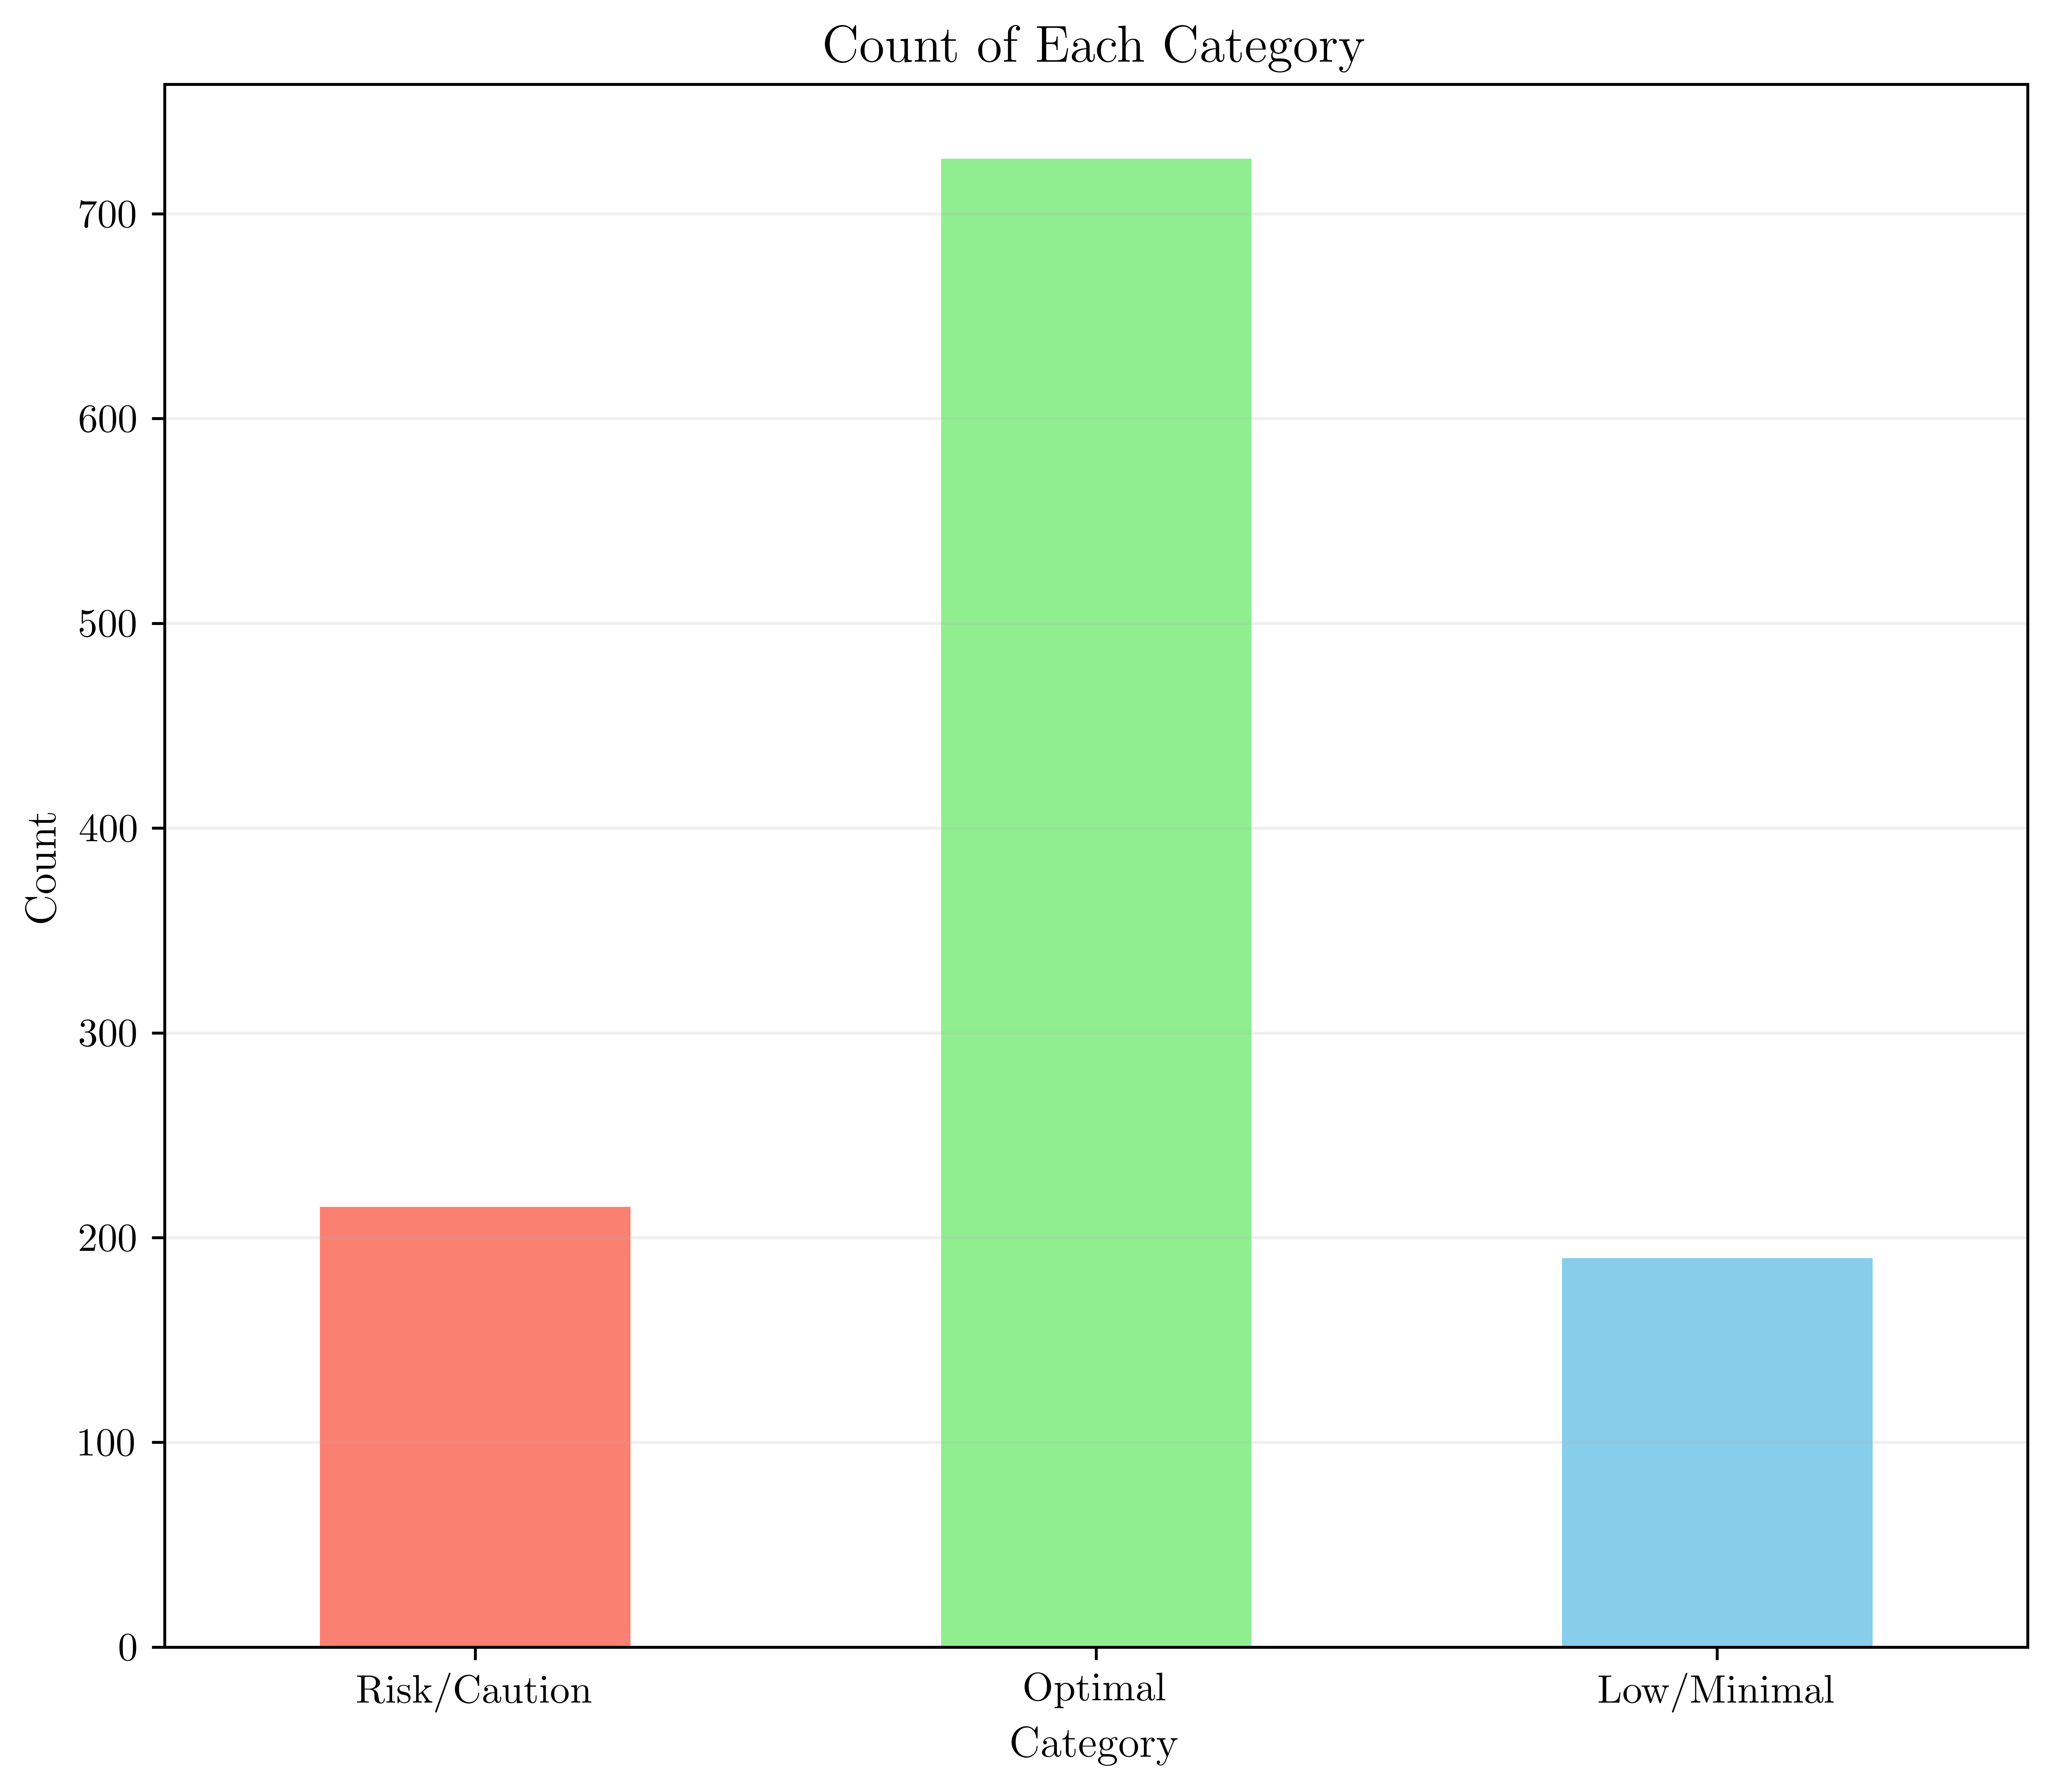
\includegraphics[width=1\linewidth]{assets/distribution_FatigInd(0).png}
    \caption{Histogram of the new classes, once 'Caution' and 'Risk' are combined in one.}
    \label{histClasses}
\end{figure}
At this stage, we opted to under sample our dataset to the number of observations of 'Risk/Caution', and over sample the observations in 'Low/Minimal', by imputing random samples from the pool of observations of 'Low/Minimal'. The use of SMOTE in this scenario would provide continuous classes for our features, which wouldn't yield any physical meaning.
To assess how the different features vary among them and in relation to the target, we computed the correlation matrix as seen in Figure~\ref{correlationMatrix}.
\begin{figure}
    \centering
    \includegraphics[width=1\linewidth]{assets/correlation_matrix_smaller.png}
    \caption{Correlation matrix of all features in the dataset}
    \label{correlationMatrix}
\end{figure}
From this we could exclude several of the features, which are verified by how the classes are distributed across the scales for each feature. Figure illustrates a proper and poor example of class distribution for a given feature.


Considering that the weights used in the dataset were identical regardless of sex, we performed some simple models in order to decide if it would be necessary to split our dataset. We could verify that gender didn't have a significant impact in model performance, so we opted to use it as a feature.
In order to keep the timeseries nature of training, increase and decrease of training intensity, and varying fatigue with training we included exponentially weighted moving averages (EWMA). This way we include memory in our model, and allow to consider the decay in the weights of events further away from any given day. The mathematical expression used to calculate EWMA for each selected feature is,
\begin{equation}
    \text{EWMA}_{\text{today}} = \text{Feature}_{\text{today}} \cdot \lambda_a + (1 - \lambda_a) \cdot \text{EWMA}_{\text{yesterday}}
\end{equation}
where $\lambda_a$ is a value between 0 and 1 that represents the degree of decay, with higher values discounting older observations at a faster rate. The $\lambda_a$ is given by:
\begin{equation}
    \lambda_a = \frac{2}{N + 1}
\end{equation} 


\begin{figure}[H]
\centering
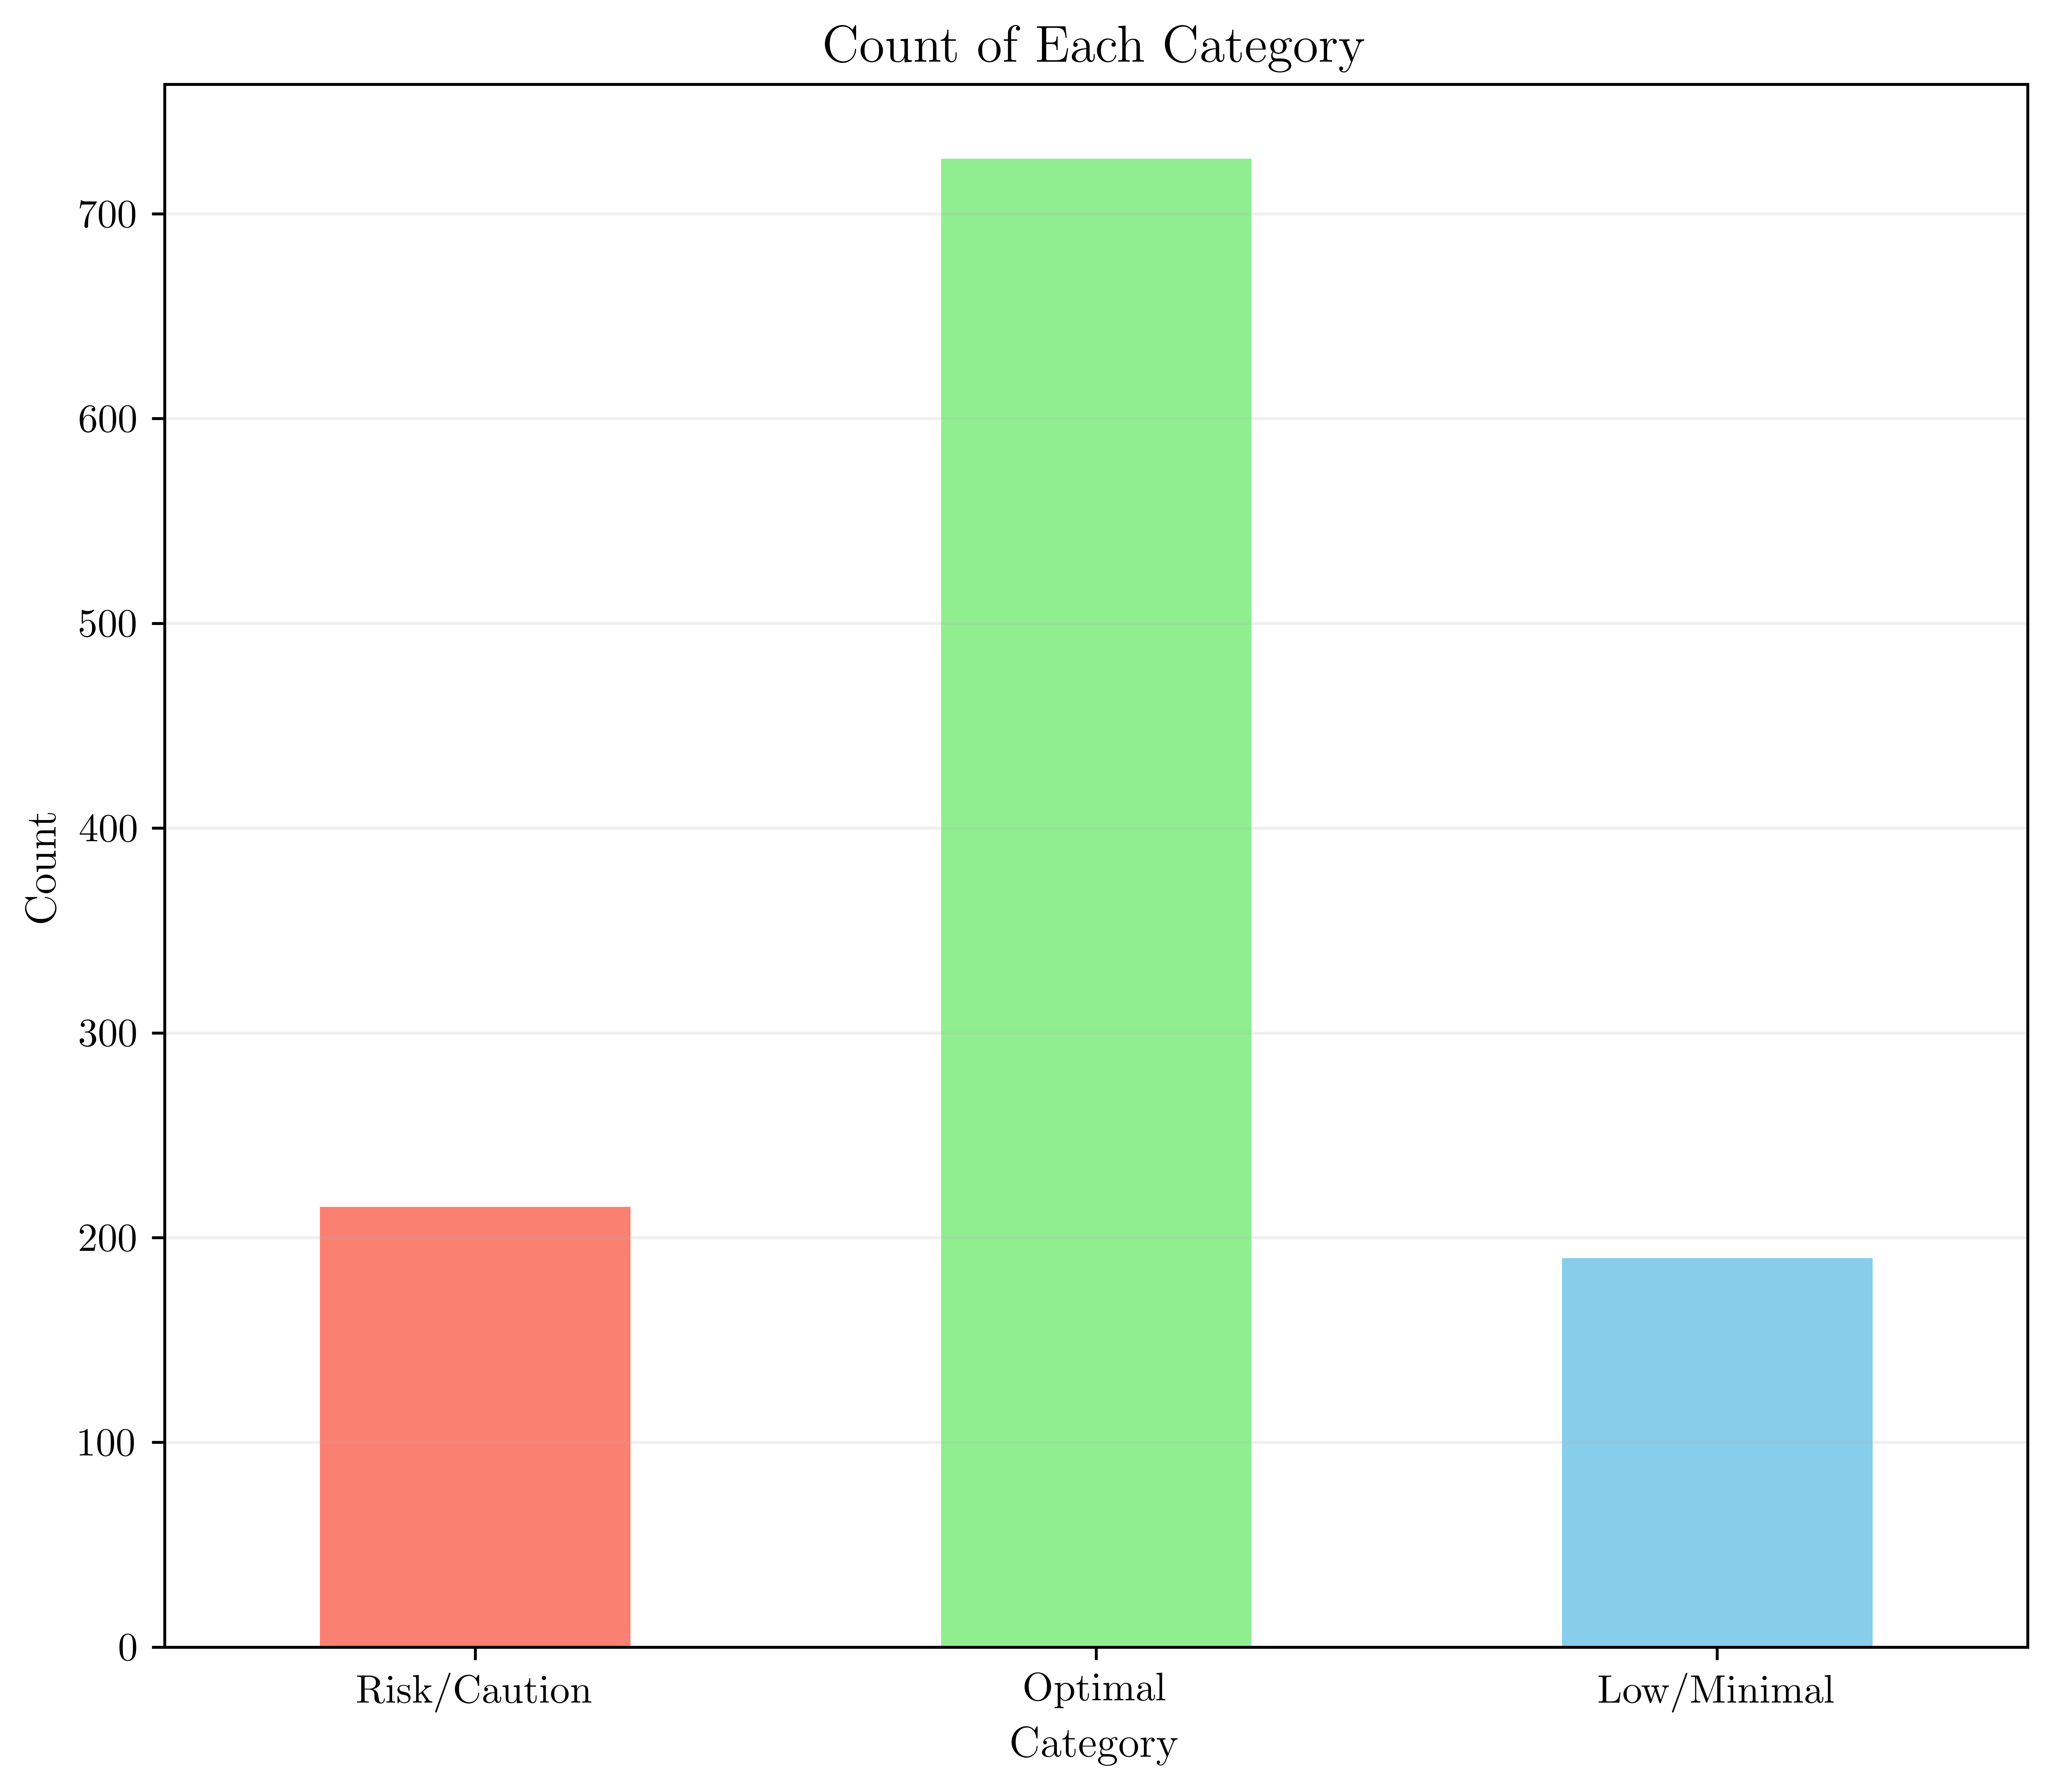
\includegraphics[width=2.5in]{assets/distribution_FatigInd(0).png}
\caption{teste grafico 2}
\label{teste_grafico}
\end{figure}

tentamos o smote mas ele criava variaveis continuas mesmo quanto eram categoricas entre outros problemas e por nao precisarmos de uma grande qnt relativa de obs geradas, ent usou se o metodo de "copiar obervacoes (procurar nome melhor)"

\begin{figure}[H]
\centering
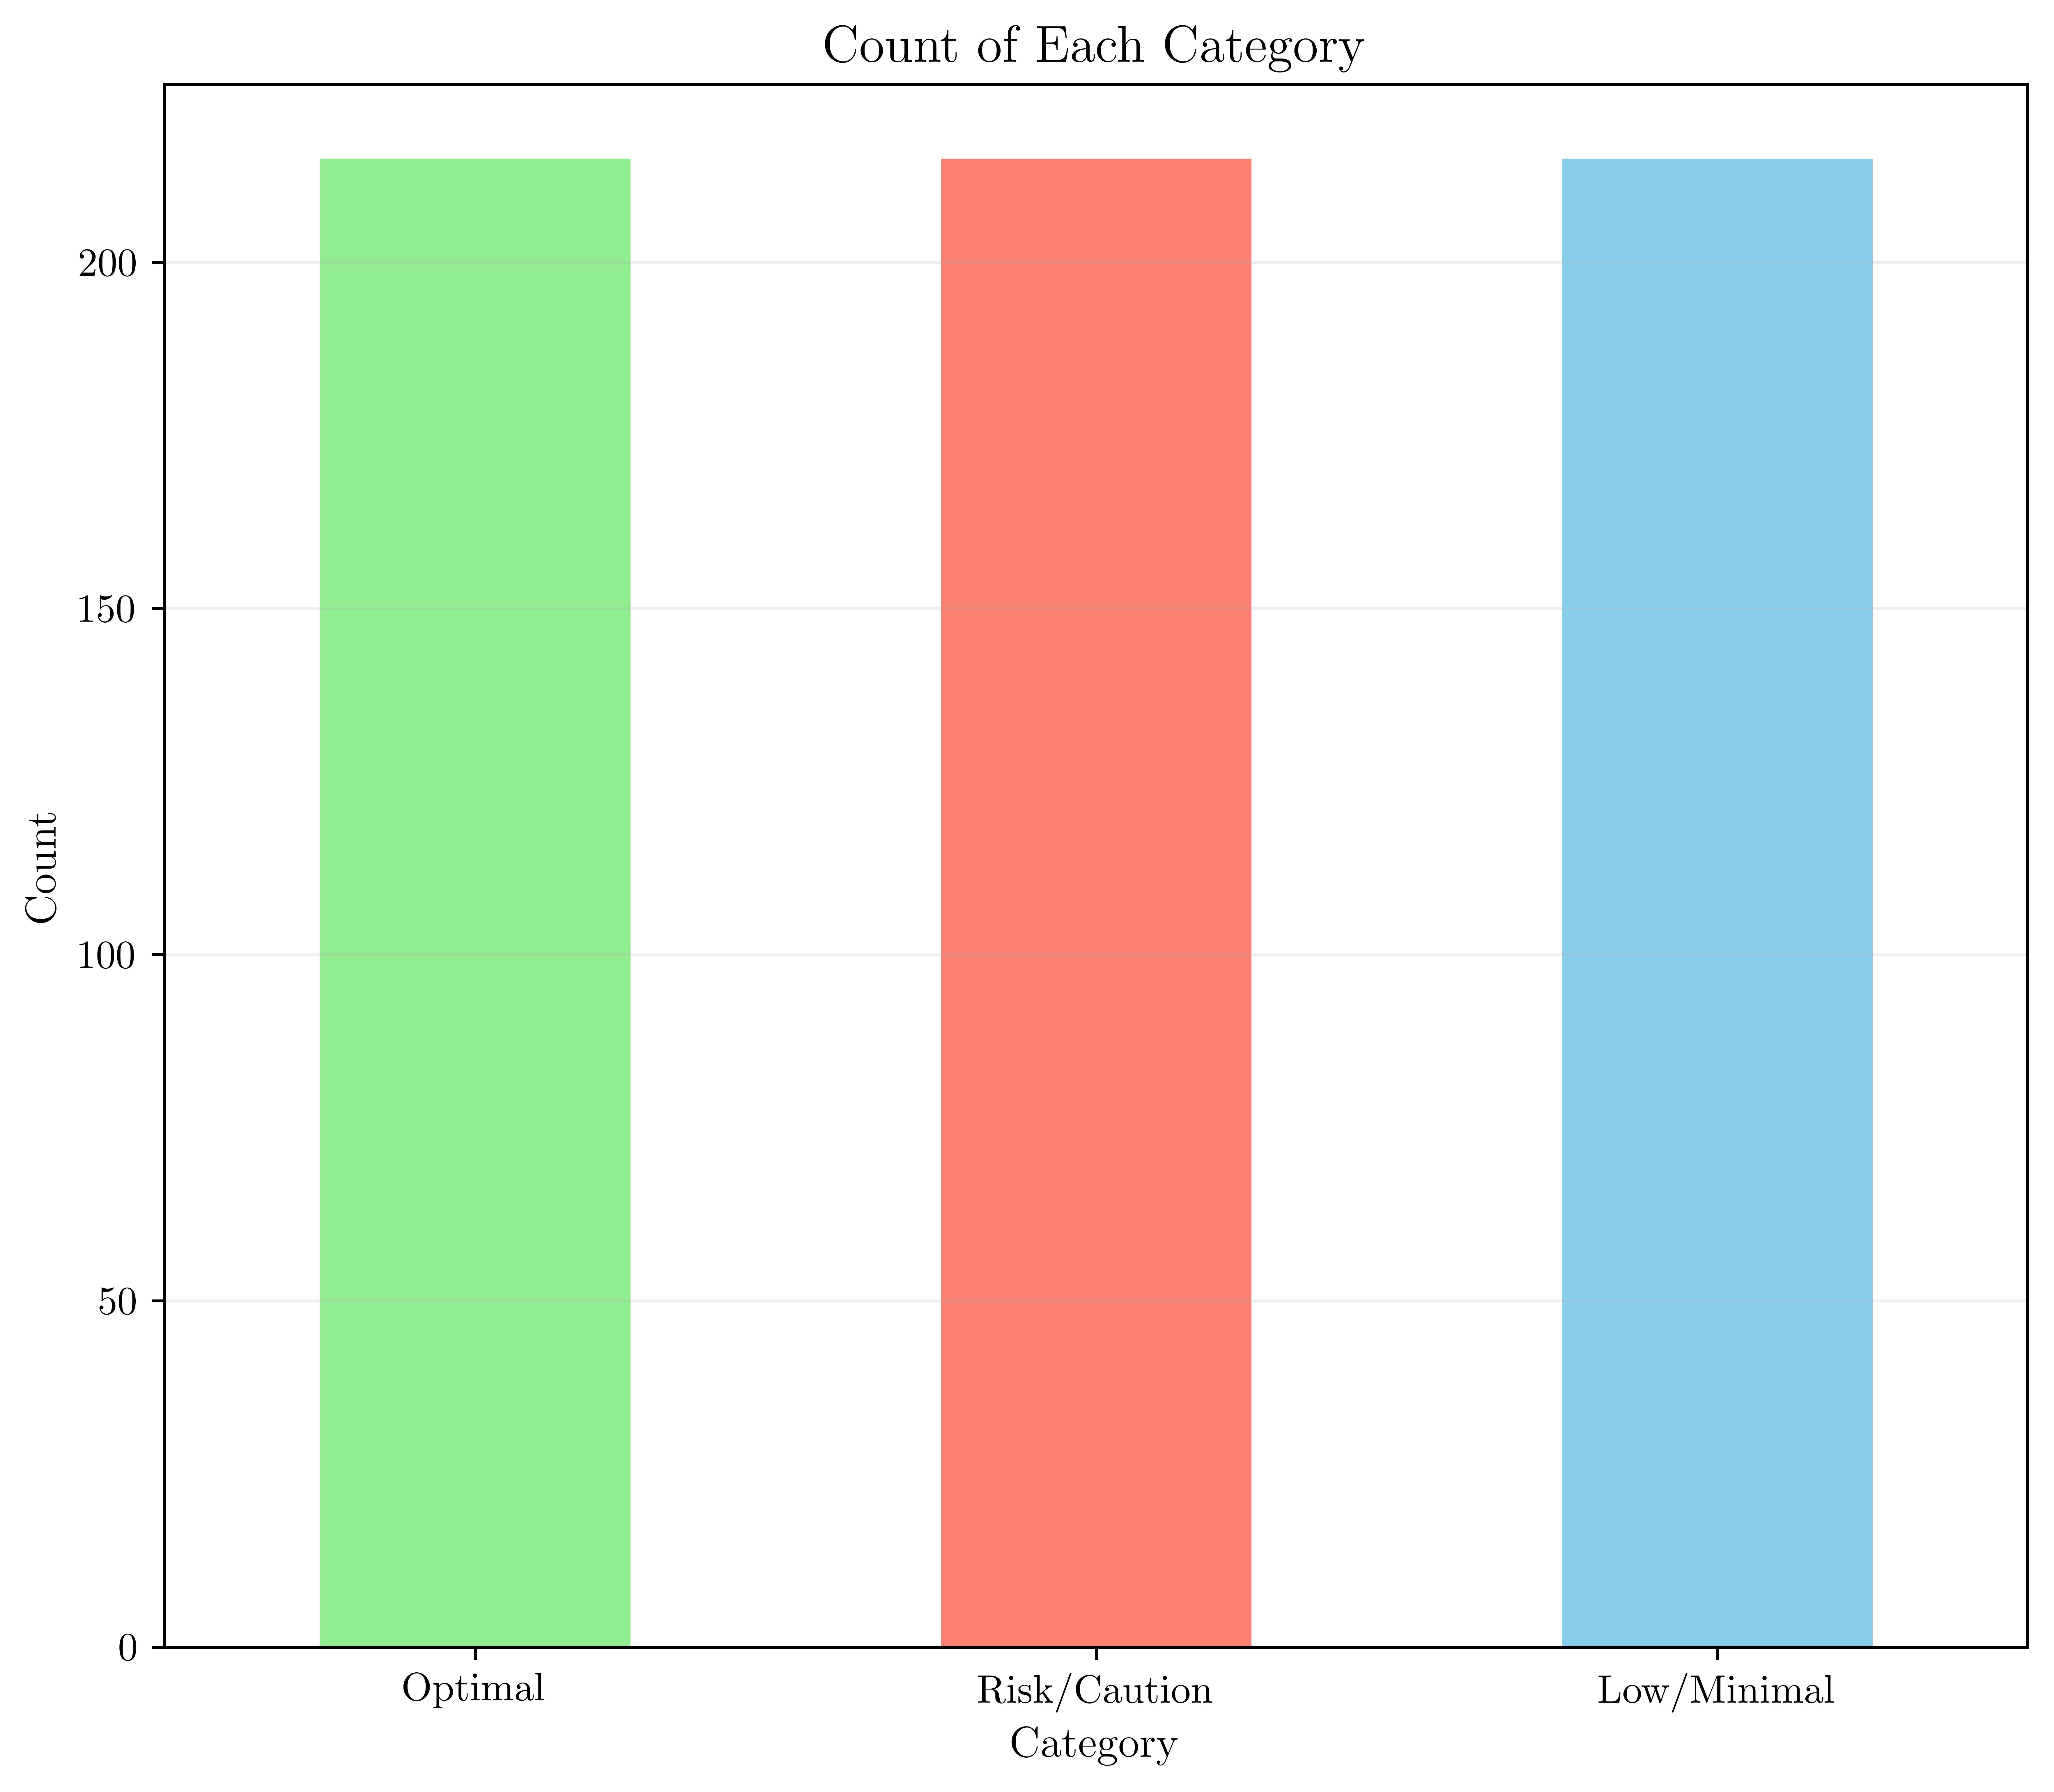
\includegraphics[width=2.5in]{assets/distribution_FatigInd(1).png}
\caption{teste grafico}
\label{teste_grafico 2}
\end{figure}

\subsection{analisa das features}

ns q temos q standartizar os dados para se tornar mais facil a sua analise, para q esteja tudo na mesma medida bla bla

foi feito uma matriz de correlacao para verificar as variaveis mais correlacionadas

foi feita uma analise bivarida? para tentar compreender padroes que hajam nos dados em relacao a nossa variavel targe, q é a fadiga

\section{classifcation models}

para classificar a fadiga, vamos usar varios modelos de machine learning tais como ......, e exprimentar variacoes dos mesmos. bla bla correcoes pesos etc

uma componente mt importante deste estudo é o avaliar cada modelo, para isso serão usadas metricas tai como ...., para analisar modelo a modelo qual é o melhor para modelas/classificar os vários niveis de fadiga

mostrar algumas formulas e graficos de exemplo etc etc

é importante reforçar tbm q todos os modelos serao treinados com 80\% acho eu e ns q o resto é teste bla bla

\subsection{modelo 1 lalala}

ns q regressao logistica bla bla, paramentros e tudo mais

foi usado a do sklearn ou assim


\subsubsection{sem termo de castigo ou assim}

ns q resultados bla bla

\subsubsection{com termo de castigo ou assim}

ns q mais resultados

meter tabelas com resultados e tudo mais, mas so no fim metemos uma geral a comparar tudo

meter:

- matriz de confusao

- precision score

- f1 score

- accuracy score

- recall score

- cross validation

- AUC (area under the curve)

\subsection{modelo 2 lalal}

ns q do sklean, funcao tal e coisa ....


\section{comparacao dos modelos}

comparar aqui todos os resultados e isso

acuracaia, learning curves, etc , etc

- learning curves

- scalability 

- performance 

- cross validation

\section{restulados}

observa se q o melhor é tal e tal, mas aquele fez isto e ns q


\section{Conclusion}
The conclusion goes here.


% An example of a double column floating figure using two subfigures.
% (The subfig.sty package must be loaded for this to work.)
% The subfigure \label commands are set within each subfloat command,
% and the \label for the overall figure must come after \caption.
% \hfil is used as a separator to get equal spacing.
% Watch out that the combined width of all the subfigures on a 
% line do not exceed the text width or a line break will occur.
%
%\begin{figure*}[!t]
%\centering
%\subfloat[Case I]{\includegraphics[width=2.5in]{box}%
%\label{fig_first_case}}
%\hfil
%\subfloat[Case II]{\includegraphics[width=2.5in]{box}%
%\label{fig_second_case}}
%\caption{Simulation results for the network.}
%\label{fig_sim}
%\end{figure*}
%
% Note that often IEEE papers with subfigures do not employ subfigure
% captions (using the optional argument to \subfloat[]), but instead will
% reference/describe all of them (a), (b), etc., within the main caption.
% Be aware that for subfig.sty to generate the (a), (b), etc., subfigure
% labels, the optional argument to \subfloat must be present. If a
% subcaption is not desired, just leave its contents blank,
% e.g., \subfloat[].


% An example of a floating table. Note that, for IEEE style tables, the
% \caption command should come BEFORE the table and, given that table
% captions serve much like titles, are usually capitalized except for words
% such as a, an, and, as, at, but, by, for, in, nor, of, on, or, the, to
% and up, which are usually not capitalized unless they are the first or
% last word of the caption. Table text will default to \footnotesize as
% the IEEE normally uses this smaller font for tables.
% The \label must come after \caption as always.
%
%\begin{table}[!t]
%% increase table row spacing, adjust to taste
%\renewcommand{\arraystretch}{1.3}
% if using array.sty, it might be a good idea to tweak the value of
% \extrarowheight as needed to properly center the text within the cells
%\caption{An Example of a Table}
%\label{table_example}
%\centering
%% Some packages, such as MDW tools, offer better commands for making tables
%% than the plain LaTeX2e tabular which is used here.
%\begin{tabular}{|c||c|}
%\hline
%One & Two\\
%\hline
%Three & Four\\
%\hline
%\end{tabular}
%\end{table}









% use section* for acknowledgment
\section*{Acknowledgment}


%The authors would like to thank... ~\cite{Author2024}


\section{NOTAS}

Considerar usar dataset com informação combinada de atletas para reter carácter temporal (progressão da época, aumento de cargas e combinação com features que tenham referência temporal [carga de treino do dia anterior]

Modelos sugeridos: Random Forest / SVM

temos com objetivo generalizar para que qq treinador possa ter nocao do comporamento e do estado dos seus atletas, podendo ajustar os seus treinos e cargas físicas consoante as medidas de fadigas.

para alem disso tbm se quer ver quais as metricas mais importantes relacionadas coma a fadiga

De acordo com a conversa com a professora é importante perceber como é que se deve definir a memória da nossa t-SNE, e a importância que isso tem no período da fadiga.

ns q dados fornecidos por um treinador de natacao, tivemos de organizar os dados em folhas de excel, visto estarem por linhas e com graficos e formulas de acordo com o treinador, bla bla, teve-se fazer oq? sabes melhor q eu pq foste tu q fizeste

os valores da fadiga foram convertidos para categoricos, pq e mais interessante classificar a fadiga, tendo em conta intervalos dados pelo treinador, do q numero que tornam mais dificl a interpretacao dos mesmos

de seguida agruparam-se os dados todos num novo ficheiro excel, para posterior analise atraves do python, de forma mais facilitata

tem se entao dados diarios, para X atletas, durante ns q tempo, ao longo da epoca tal, totalizando x observacoes (linhas)

para cada observacao tem se variaveis como ... bla bla e bla, contudo, nem todas serao usadas, devido a insights dados pelo treinador aka expert

as variaveis que irao ser utilizadas no estudo são tal tal, que representa tal, tal tal, ... ns q ns q mais.




% trigger a \newpage just before the given reference
% number - used to balance the columns on the last page
% adjust value as needed - may need to be readjusted if
% the document is modified later
%\IEEEtriggeratref{8}
% The "triggered" command can be changed if desired:
%\IEEEtriggercmd{\enlargethispage{-5in}}


\bibliographystyle{IEEEtran}
\bibliography{references}
\begin{thebibliography}{99}
\bibitem{example} A. Author, "Title of the paper," Journal Name, vol. 12, no. 3, pp. 45--67, 2024.
\end{thebibliography}

\end{document}



